\chapter{Transformers}
\textbf{Transformer} were initially targeted at natural language processing (NLP)
problems, where the network input is a series of high-dimensional embeddings
representing words or word fragments. This architecture was designed with the goal
of processing this text into a representation suitable for downstream tasks.

We can also encounter different problems such as:
\begin{itemize}
    \item The encoded input can be very large. Assuming a 1024-d embedding and
          body of text that have 100s/1000s of words, a fully connected neural
          network is impractical because we have $100 \times 1024 = 102400$ as
          input length;
    \item Each input is of different length and Feed Forward Neural Networks are
          impracticable;
    \item Statistics are similar at every position;
    \item The language is fundamentally ambiguous.
\end{itemize}

Most of these problems are derived by NLP problems.
\section{Dot-product self attention}
Considering the issues just presented, we want to design a network that is able
to process text and can:
\begin{enumerate}
    \item Use parameter sharing to cope with long input passages of differing
          lengths;
    \item Contain connections between word representations that depend on the
          words themselves.
\end{enumerate}
The transformer acquires both properties by using \textbf{Dot-Product Self-Attention}.
This mechanism is shown in Figure \ref{fig:sa}.

\begin{figure}[!ht]
    \centering
    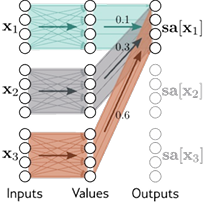
\includegraphics[width=0.3\linewidth]{img/transformer/selfattention.png}
    \caption{Dot-Product Self-Attention mechanism}
    \label{fig:sa}
\end{figure}

While a standard NN layer $f[x]$ takes a $D\times 1$ input $x$ and applies a
linear transformation followed by a non-linear activation function $a[\cdot]$:
\begin{equation*}
    f[x] = a[\beta + \Omega x]
\end{equation*}
where $\beta$ contains the biases and $\Omega$ contains weights. A self-attention
block $sa[\cdot]$ takes $N$ inputs $x_n$, each of dimension $D \times 1$, and
returns $N$ output vectors of the same size. In the context of NLP each $x_n$
will represent a word or a word fragment of a sentence.

Let's go into more detail. First, a set of \textbf{values} are computed for each
input:
\begin{equation}
    v_n = \beta_v + \Omega_v \cdot x_n
\end{equation}
where $\beta_v$ contains the biases and $\Omega_v$ contains the weights. Then the
$n$-th output $sa[x_n]$ is a weighted sum of all the values $v_n$:
\begin{equation}
    sa[x_n] = \sum_{m = 1}^N a[x_m, x_n] \cdot v_m
\end{equation}
The scalar weight $a[x_m, x_n]$ is the \textbf{attention} that input $x_n$ pays
to input $x_m$. The $N$ weights $a[\cdot, x_n]$ are non-negative and sum to one.

Self-attention can be understood as a mechanism that routes the values in different
proportions to construct each output.

To compute the values, the same weights $\Omega_v$ ($D \times D$) and biases
$\beta_v$ ($D \times 1$) are applied to each input $x_n$ ($D \times 1$):
\begin{equation}
    v_n = \beta_v + \Omega_v \cdot x_n
\end{equation}
This computation scales linearly with the sequence length $N$, so it requires less
parameters than a fully connected neural network connecting all $DN$ inputs to
the $DN$ outputs.

The value computation can thus be viewed as a sparse matrix multiplication (see
Figure \ref{fig:valuesComputation}) with shared parameters.
\begin{figure}[!ht]
    \centering
    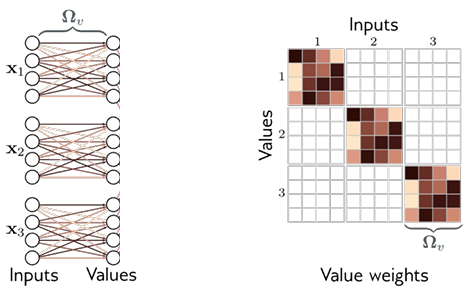
\includegraphics[width=0.5\linewidth]{img/transformer/values.png}
    \caption{Values computation in self-attention using shared parameters}
    \label{fig:valuesComputation}
\end{figure}

The attention weights $a[x_m, x_n]$ combine the values from different inputs. They
are also sparse (Figure \ref{fig:attention}), since there is only one weight for
each ordered pair of inputs $(x_m, x_n)$regardless of the size of these inputs.

\begin{figure}[!ht]
    \centering
    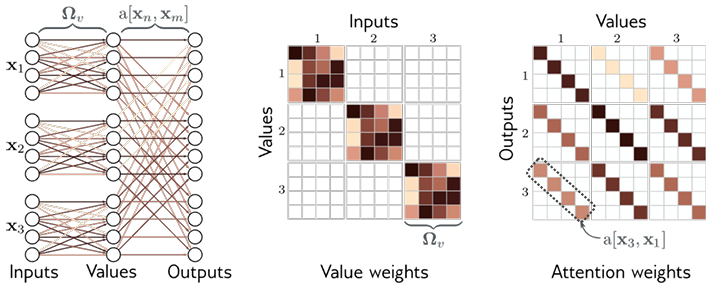
\includegraphics[width=0.6\linewidth]{img/transformer/attention.png}
    \caption{Attention}
    \label{fig:attention}
\end{figure}

The number of attention weights has a quadratic dependence on the sequence length
$N$ but it is independent of the length $D$ of each input $x_n$.

Through this process, you get the same output as that from two-chained linear
transformations:
\begin{itemize}
    \item The value vectors are computed independently from each input;
    \item and these vectors are linearly combined by the attention weights.
\end{itemize}

However, the overall self-attention is non-linear because the attention weights
are themselves non-linear functions of the input. This is an example of a
\textbf{hypernetwork}, where one network branch computes the weights of another
branch.

To compute the \textit{attention}, we apply two more linear transformations to
the inputs:
\begin{equation}
    q_n = \beta_q + \Omega_q \cdot x_n \,\,\, \land \,\,\, k_n = \beta_k + \Omega_k \cdot x_n
\end{equation}
where $q_n$ and $k_n$ are referred to as the \textbf{queries} and the \textbf{keys}.

We then compute dot products between the queries and the keys followed by a softmax:
\begin{equation}
    a[x_m, x_n] = softmax_m [k_\ast^T, q_n] = \frac{\exp[k_\ast^T, q_n]}{\sum_{m' = 1}^N \exp[k_\ast^T, q_n]}
\end{equation}
so, for each $x_n$ they are positive and sum to one and these is the method to apply
non linearity on attention.

The names \textit{queries} and \textit{keys} have the following interpretation:
\begin{itemize}
    \item The dot-product operation returns a measure of similarity between its
          inputs, so the weights $a[x_\ast, x_n]$ depend on the relative similarities
          between each query and the keys;
    \item The softmax function means that we can think of the key vectors as
          \textit{competing} with one another to contribute to the final result.
\end{itemize}
The queries and keys must have the same dimensions.

However, these can differ from the dimension of the values, which is usually the
same size as the input, so that the representation does not change size.

This mechanism fulfills the initial requirements:
\begin{enumerate}
    \item There is a single shared set of parameters $\phi = \{\beta_v, \Omega_v,
              \beta_q, \Omega_q, \beta_k, \Omega_k\}$. This is independent of the
          number of inputs $N$, so the networks can be applied to difference
          sequence lengths;
    \item There are connections between the inputs (words), and the strength of
          these connections depends on the inputs themselves via the attention weights.
\end{enumerate}

This can be written in a compact form if the $N$ inputs $x_n$ form the columns of
the $D \times N$ matrix $X$. The values, queries, and keys can be computed as:
\begin{align*}
    V[X] = \beta_v \cdot 1^T + \Omega_v \cdot X \\
    Q[X] = \beta_q \cdot 1^T + \Omega_q \cdot X \\
    K[X] = \beta_k \cdot 1^T + \Omega_k \cdot X
\end{align*}
The self-attention computation is then:
\begin{equation}
    sa[X] = V[X] \cdot softmax[K[X]^T, Q[X]]
\end{equation}
where softmax is independently applied on the columns of its input.

Since the dot-product in the attention calculation can result in large magnitudes,
it pushes the arguments of the softmax function into a region where the largest
value dominates entirely. This causes small changes to the softmax inputs to
have minimal impact on the output, making the model harder to train.

To mitigate this, the dot products are scaled by the square root of the size of
the query $D_q$ and key $D_k$, which corresponds to the number of rows in $\Omega_q$
and $\Omega_k$ as the query and key dimensions must be the same.
\begin{equation}
    sa[X] = V \cdot softmax\left[\frac{K^T \cdot Q}{\sqrt{D_q}}\right]
\end{equation}

\section{Positional encoding}
The self-attention mechanism discards important information, in fact, the computation
is the same regardless of the order of the inputs. However, the order is important
when the inputs correspond to the words in a sentence. There are two main approaches
to incorporating position information:
\begin{itemize}
    \item \textbf{Absolute position embeddings};
    \item \textbf{Relative position embeddings}.
\end{itemize}
\subsection{Absolute position embeddings}
This method consists of adding a $\Pi$ matrix to the $X$ input. The purpose of
this matrix is to encode positional information. Each column of $\Pi$ is unique
and contains information about the absolute position in the input sequence.

The matrix that is usually used for this purpose can be handcrafted or learned in
the model training phase. Typically, this matrix is added to the model's input.
Alternatively, since the outputs of the self-attention blocks have the same dimensions
as the input, the matrix can be added after each layer.

\begin{note}
    Sometimes it is added to $X$ in the computation of the queries and keys but
    not to the values.
\end{note}

\subsection{Relative position embeddings}
In this case, we are considering a situation where the input to a self-attention
mechanism may be an entire sentence, many sentences, or just a fragment of a sentence,
and the absolute position of a word is much less important than the relative
position between two inputs. Of course, this can be recovered if the system knows
the absolute position of both, but relative position embeddings encode this
information directly. Each element of the attention matrix corresponds to a
particular offset between query position $a$ and key position $b$.

Relative position embeddings learn a parameter $\pi_{a, b}$, for each offset and
use this to modify the attention matrix by adding these values, multiplying by them,
or using them to alter the attention matrix in some other way.
\section{Multiple heads self attention}
In the most used architectures, multiple self-attention mechanisms are used in
parallel, and this is known as \textbf{Multi-Head Self-Attention}. If we now
consider the fact of having $H$ self-attention blocks, we have that the different
sets of values, keys and queries are calculated as:
\begin{align*}
    V_h[X] = \beta_{vh} \cdot 1^T + \Omega_{vh} \cdot X \\
    Q_h[X] = \beta_{qh} \cdot 1^T + \Omega_{qh} \cdot X \\
    K_h[X] = \beta_{kh} \cdot 1^T + \Omega_{kh} \cdot X
\end{align*}
Then, the $h-$th self-attention mechanism or \textbf{head} can be written as:
\begin{equation}
    sa_h[X] = V_h \cdot softmax\left[\frac{K_h^T \cdot Q_h}{\sqrt{D_q}}\right]
\end{equation}
where we have different parameters for each head.

Typically, if the dimension of the inputs $x_m$ is $D$ and there are $H$ heads,
the values, queries, and keys will all be of size $D / H$ as this allows for an
efficient implementation. The outputs of these self-attention mechanisms are then
vertically concatenated, and another linear transform $\Omega_c$ is applied to
combine them. An example with $H = 2$ is shown in Figure \ref{fig:multiHead}.
The output of the multi-head self-attention mechanism is then:
\begin{equation}
    Mhsa[X] = \Omega_c[sa_1[X]^T, sa_2[X]^T, \dots, sa_H[X]^T]
\end{equation}
\begin{figure}[!ht]
    \centering
    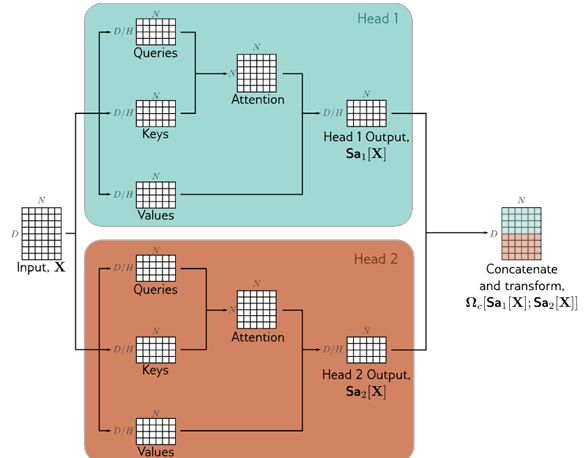
\includegraphics[width=0.5\linewidth]{img/transformer/multihead.png}
    \caption{Multi-Head Self-Attention example with $H = 2$}
    \label{fig:multiHead}
\end{figure}

This last transformation is useful because it allows to bring the weights of the
different heads in the same range. In addition, if necessary, this combination
can be used to limit a head that provides wrong data in output by setting it to
zero.

Multiple heads seem to be necessary to make the transformer work well. It has
been speculated that they make the self-attention network more robust to bad
initializations.

\section{Transformer Layers}
All the components we have defined so far serve as a basis for defining the
\textbf{Transformer Layer}. This is the basic building block of the transformer
architecture. The structure of a Transformer Layer is shown in Figure \ref{fig:transformerLayers}.

\begin{figure}[!ht]
    \centering
    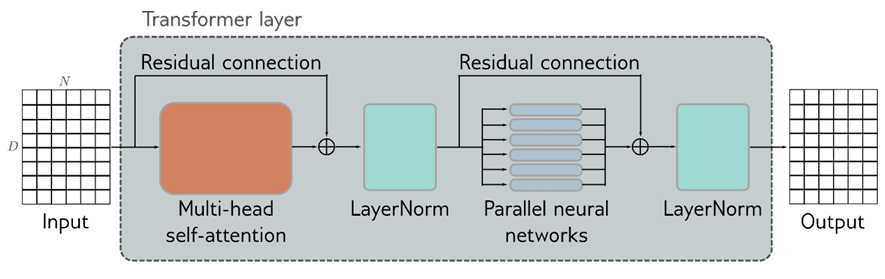
\includegraphics[width=0.5\linewidth]{img/transformer/transformerlayers.png}
    \caption{Transformer Layers}
    \label{fig:transformerLayers}
\end{figure}

Transformer Layer consists of a multi-head self-attention unit, which allows the
word representations to interact with each other, followed by a fully connected
network $mlp[x_\ast]$ that operates separately on each word. Both units are
residual networks.

In addition, it is typical to add a \textbf{LayerNorm} operation after both the
Self-Attention and Fully Connected Networks.

Architecture that are now used in practice are more complex in the sense that
they have more than one layer of self-attention and fully connected networks.

\section{NLP pipeline}
A typical NLP pipeline begins with a \textbf{tokenizer}, which splits text into
a vocabulary of smaller constituent units (tokens) that the subsequent network
can process. These tokens often represent words, but several challenges arise:
\begin{itemize}
    \item Inevitably, some words (e.g., names) will not be present in the vocabulary;
    \item Handling punctuation can be unclear, yet crucial. For example, if a
          sentence ends with a question mark, this information must be encoded;
    \item The vocabulary would require separate tokens for different forms of the
          same word (e.g., variations with different suffixes), with no mechanism
          to clarify that these variations are related.
\end{itemize}

Each of these tokens is mapped to a learned embedding. These embeddings are then
passed through a series of transformer layers. We will now examine each of these
stages in detail.

In practice, a compromise between letters and full words is employed. The final
vocabulary includes both common words and word fragments, which can be combined
to represent larger and less frequent words. This vocabulary is typically generated
using a sub-word tokenizer, such as byte pair encoding (BPE), which greedily merges
frequently occurring substrings based on their frequency.

Each token in the vocabulary $\mathcal{V}$ is consistently mapped to a corresponding
word embedding, ensuring that the same token always maps to the same embedding.

To accomplish this, the $N$ input tokens are represented in the matrix $T$, with
dimensions $|V| \times N$. Each column of $T$ corresponds to a token, where the
$n$-th column represents the $n$-th token as a one-hot vector of size $|V| \times 1$.

The embeddings for the entire vocabulary are stored in a matrix $\Omega_e$, with
dimensions $D \times |V|$. The input embeddings are computed as $X = \Omega_e \cdot T$,
where $\Omega_e$ is learned like any other parameter of the network.

A typical embedding size $D$ is 1024, and a typical vocabulary size $|V|$ is 30,000.
As a result, even before the main network processes the data, the matrix $\Omega_e$
contains a large number of parameters to learn.

Finally, the embedding matrix $X$, which represents the text, is passed through
a series of transformer layers, forming what is known as a transformer model.


There are three types of transformer models:
\begin{enumerate}
    \item \textbf{Encoders}: An encoder transforms text embeddings into representations
          that support a variety of tasks. \textbf{BERT} (Bidirectional Encoder
          Representations from Transformers) is an example of an encoder model
          with a vocabulary of 30,000 tokens. Input tokens are mapped to 1,024-dimensional
          word embeddings and processed through 24 transformer layers, each
          containing a self-attention mechanism with 16 heads. Each head computes
          queries, keys, and values with a dimension of 64. Encoder models like
          BERT employ transfer learning. During pretraining, the transformer's
          parameters are learned via self-supervision on a large text corpus. The
          pretraining objective is to capture general statistical knowledge of
          language through tasks such as predicting missing words in sentences.
          The learned text representations can then be fine-tuned for specific
          NLP tasks.
    \item \textbf{Decoders}: A decoder generates new tokens to extend an input
          text sequence. For example, \textbf{GPT-3} constructs an autoregressive
          language model, where the joint probability of a sequence of tokens
          $(t_1, t_2, \dots, t_N)$ is factored as:
          \begin{equation}
              P(t_1, t_2, \dots, t_N) = P(t_1) \cdot \prod_{n=2}^N P(t_n \mid t_1, \dots, t_{n-1})
          \end{equation}
          This autoregressive approach defines a probability distribution over
          text sequences, enabling the generation of new, coherent text. Given an
          input sequence, the model predicts a probability distribution over
          possible next tokens. The selected token is appended to the sequence and
          fed back into the model, repeating the process iteratively to generate
          text.
    \item \textbf{Encoder-Decoders}: Encoder-decoder models are designed for
          sequence-to-sequence tasks, such as \textbf{machine translation}, where
          text in one language is transformed into another. These models encode
          the input sequence into a latent representation and decode it into the
          target sequence.
\end{enumerate}